\documentclass[a4paper,class=article,border=10pt,tikz]{standalone}
\usepackage{tikz}
\usetikzlibrary{snakes,calc,positioning,patterns,angles,quotes,decorations.pathmorphing,decorations.markings,through}
\usetikzlibrary{arrows,decorations,decorations.text}
\usepackage{rotating}
\usetikzlibrary{arrows,decorations,decorations.text}
\usetikzlibrary{patterns.meta,math}




\usepackage{siunitx}

\begin{document}

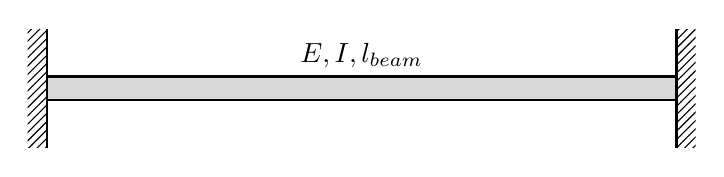
\begin{tikzpicture}

    \tikzstyle{ground}=[fill,pattern=north east lines,draw=none,minimum width=0.75cm,minimum height=0.3cm]
     \tikzstyle{close}=[draw=none,minimum width=0.75cm,minimum height=0.3cm]
    \tikzstyle{spring}=[thick,decorate,decoration={zigzag,pre length=0.3cm,post length=0.3cm,segment length=0.3cm}]
    \tikzstyle{force}=[>=stealth',ultra thick]

      \coordinate (origo) at (0,0);




    \node (part1) [draw,fill=gray!30,outer sep=0pt,thick,minimum width=8cm, minimum height=0.3cm,anchor=east,label={above:{}}] at (origo){};
    \node (p1_label) at ($(part1) + (0,0.7)$) [below] {$E, I,l_{beam}$};

\node (wall_1) [ground,minimum width=0.2cm, minimum height=1.5cm,anchor=east] at (part1.west) {};

\draw [thick] (wall_1.north east) -- (wall_1.south east);


\node (wall_2) [ground,minimum width=0.2cm, minimum height=1.5cm,anchor=west] at (part1.east) {};

\draw [thick] (wall_2.north west) -- (wall_2.south west);

 
\end{tikzpicture}


\end{document}
